%%%%%%%%%%%%%%%%%%%%%%%%%%%%%%%%%%%%%%%
%%% VALORES INICIAIS
%   Geracao de valores iniciais para o PNC. Condicionamento
%   de integrais primeiras, condições de Hénon, distribuições
%   para massas, posições e momentos.
%%%%%%%%%%%%%%%%%%%%%%%%%%%%%%%%%%%%%%%
\section{Valores iniciais}\label{secao:valores_iniciais}

O programa foi elaborado de modo que é possível entrar com valores iniciais de duas maneiras: diretamente e através de sorteios. Da primeira forma, é necessário informar cada massa, posição e momento linear inicial para cada corpo, o que é prático para problemas de poucos corpos mas inviável, a priori, conforme $N$ cresce, sendo necessário utilizar da segunda forma. Vale ressaltar que o sorteio também gera um arquivo de valores iniciais, então a primeira forma pode ser utilizada a posteriori.

Para gerar valores iniciais aleatórios é preciso escolher critérios que atendam as necessidades do problema que se objetiva simular. Para além de gerar valores utilizando, por exemplo, uma distribuição uniforme, muitas vezes é necessário também condicionar os valores gerados de modo que atendam determinada demanda, como os valores das integrais primeiras ou critérios iniciais para um sistema poder ser estável ou não. Tratamos esses dois casos a seguir.

%%%%%%%%%%%%%%%%%%%%%%%%%%%%%%%%%%%%%%%%%%%%%%%%%%%%
\subsection{Condicionamento das integrais primeiras}
Considere valores iniciais $(\vet m, \vet q, \vet p) \in \R_+^N \times \R^{3N} \times \R^{3N}$ obtidos através de um gerador com uma distribuição de probabilidade qualquer, que tenha integrais primeiras $E$, $\vet J$, $\vet P$ e $\vet G$, sendo $\vet G(t) = M \vet q_{cm} (t) - t \vet P$.

Começando por $\vet G$, é importante lembrar que o PNCG tem equações de movimento autônomas, então no instante inicial tem-se $\vet G = M \vet q_{cm}$. Assim, para obter $\tilde{\vet G}$ desejado basta que
\begin{equation*}
    \vet q_{cm}(0) = \dfrac{1}{M} \tilde{\vet G},
\end{equation*}
e para obter tal centro de massas basta transladar as coordenadas $\vet q_a$ individualmente:
\begin{equation*}
    \tilde{\vet q_a} = \vet q_a - \dfrac{1}{M} \left(\vet q_{cm}(0) - \tilde{\vet G}\right).
\end{equation*}

Como já dito anteriormente, o PNCG também é invariante por translações, uma vez que o potencial $V$ o é. Isso significa que utilizar como condição inicial $\vet q$ ou $\tilde{\vet q}$ não afeta a forma como o sistema evoluirá. Assim, uma facilidade bastante conveniente, como já feito anteriormente, é começar com o centro de massas na origem:
\begin{equation}\label{eq:condicionamento_rcm}
    \tilde{\vet q_a} = \vet q_a - \dfrac{1}{M} \vet q_{cm}(0)
    \Rightarrow
    \tilde{\vet G} = \vet 0.
\end{equation}

No caso de $\vet P$, para gerar um $\tilde{\vet P}$ é necessário obter $\tilde{\vet p}$ tal que $\tilde{\vet P} = \sum_{a=1}^{N} \tilde{\vet p_a}$. Então:
\begin{equation*}
    \tilde{\vet P} 
    = \vet P - \vet P + \tilde{\vet P}
    = \sum_{a=1}^{N} \vet p_a - \dfrac{c_a}{C}\left(\vet P - \tilde{\vet P}\right),
    \quad
    C = \sum_{a=1}^{N} c_a,
    \quad
    c_a > 0, \forall a.
\end{equation*}
As constantes $c_a$ podem ser quaisquer, correspondendo a pesos atribuídos a cada momento linear. No caso do PNCG, uma escolha conveniente de pesos é a massa de cada corpo, sendo então
\begin{equation}\label{eq:condicionamento_p}
    \tilde{\vet p_a} = \vet p_a - \dfrac{m_a}{M} (\vet P - \tilde{\vet P}).
\end{equation}

Para o momento angular total $\vet J$, embora para problemas planares baste aplicar 
\begin{equation*}
    \tilde{\vet p_a} = \vet p_a - \dfrac{m_a}{I} \vet q_a \times (\vet J - \tilde{\vet J})
\end{equation*}
para obter $\tilde{\vet J}$, no caso geral em três dimensões a situação é mais complicada. 

\begin{figure}
    \centering
    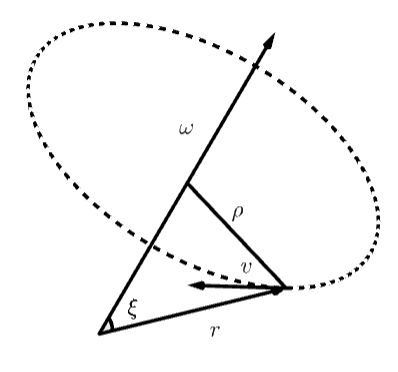
\includegraphics[width=0.3\linewidth]{tcc//img/rotacao.png}
    \caption{Situação descrita.}
    \label{fig:angular_rotacao}
\end{figure}

Considere uma partícula com posição $\vet r$ e um vetor $\vet \omega$ que define um eixo de rotação, do qual $\vet r$ se distancia em $\vet \rho$ e forma um ângulo $\xi$ e cuja velocidade da partícula a relação a é $\vet v$, como na figura \ref{fig:angular_rotacao}. Nessa situação, temos que $\norma{\vet v} = \rho \norma{\vet \omega}$ e $\sin \xi = \rho / \norma{\vet r}$. Uma vez que $\vet v \perp \vet \omega$ e $\vet v \perp \vet r$, podemos concluir que $\vet v \parallel \vet r \times \vet \omega$. Mais ainda, temos que:
\begin{equation*}
    \norma{\vet r \times \vet \omega} 
    = \norma{\vet r} \norma{\vet \omega} \sin \xi
    = \rho \norma{\vet \omega} = \norma{\vet v},
\end{equation*}
então
\begin{equation}\label{eq:velocidade_angular}
    \vet v = \vet r \times \vet \omega.
\end{equation}

O momento angular $\vet J$ também é um vetor perpendicular a $\vet r$ e a $\vet v$, mas $\vet J$ e $\vet \omega$ só são colineares quando $\vet r \perp \vet \omega$. Porém, a partir de (\ref{eq:velocidade_angular}), tem-se que $\vet J = m \vet r \times (\vet r \times \omega)$, então é possível construir um operador $\vet I: \R^3 \to \R^3$ a partir de $m$ e $\vet r$ que leva $\vet \omega$ em $\vet J$ como segue. Veja que
\begin{equation*}
    \vet r \times \vet \omega = (r_2 \omega_3 - r_3 \omega_2) \hat e_1 + (r_3 \omega_1 - r_1 \omega_3) \hat e_2 + (r_1 \omega_2 - r_2 \omega_1) \hat e_3,
\end{equation*}
então
\begin{align*}
    \vet J = m \vet r \times (\vet r \times \vet \omega) &=
    m \begin{bmatrix}
        r_2 r_1 \omega_2 - r_2^2 \omega_1 - r_3^2 \omega_1 + r_1 r_3 \omega_3 \\
        r_3 r_2 \omega_3 - r_3^2 \omega_2 - r_1^2 \omega_2 + r_1 r_2 \omega_1 \\
        r_1 r_3 \omega_1 - r_1^2 \omega_3 - r_2^2 \omega_3 + r_2 r_3 \omega_2
    \end{bmatrix} \\ &=
    m \begin{bmatrix}
        -(r_2^2 + r_3^2) & r_1 r_2 & r_1 r_3 \\
        r_1 r_2 & -(r_1^2 + r_3^2) & r_2 r_3 \\
        r_1 r_3 & r_2 r_3 & - (r_1^2 + r_2^2)
    \end{bmatrix}
    \begin{bmatrix}
        \omega_1 \\ \omega_2 \\ \omega_3
    \end{bmatrix}
    := \vet I \vet \omega.
\end{align*}

Tal aplicação $\vet I$ já é bem conhecida na literatura pelo nome de \textit{tensor de inércia}, fornecendo uma nova expressão para o momento angular. No caso de diversos corpos, a ideia é definir um eixo de rotação comum e a partir dele aplicar transformações sobre a velocidade angular de cada corpo. A primeira parte é simples, pois
\begin{equation*}
    \vet J = \sum_{a=1}^{N} \vet J_a = \sum_{a=1}^{N} \vet I_a \vet \omega = \vet I_{total} \vet \omega.
\end{equation*}

A partir disso, para obter um momento angular desejado $\tilde{\vet J}$ basta encontrar um eixo $\vet \omega$ tal que
\begin{equation*}
    \vet I_{total} \vet \omega = \vet J - \tilde{\vet J}
\end{equation*}
e aplicar a transformação
\begin{equation}\label{eq:condicionamento_j}
    \tilde{\vet p_a} = \vet p_a - m_a \vet q_a \times \vet \omega.
\end{equation}

A essa altura, é natural suspeitar que aplicar (\ref{eq:condicionamento_j}) depois de (\ref{eq:condicionamento_p}) mudaria o valor de $\tilde{\vet P}$ e vice-versa. Porém, considere o misto das aplicações:
\begin{equation}\label{eq:condicionamento_j_p}
    \tilde{\vet p_a} = \vet p_a - \dfrac{m_a}{M}(\vet P - \tilde{\vet P}) - m_a \vet q_a \times \omega.
\end{equation}

Temos:
\begin{align*}
    \sum_{a=1}^{N} \tilde{\vet p_a}
    & = \tilde{\vet P} - \vet q_{cm} \times \omega = \tilde{\vet P}
    \\
    \sum_{a=1}^{N} \vet q_a \times \tilde{\vet p_a}
    & = \tilde{\vet J} - \dfrac{1}{M} \vet q_{cm} \times (\vet P - \tilde{\vet P}) = \tilde{\vet J},
\end{align*}
pois $\vet q_{cm} = \vet 0$. Assim, com o centro de massas na origem, é possível condicionar o momento linear total e o momento angular total separadamente.

Já para a energia total $E$, existem dois caminhos possíveis: aplicar transformações sobre as posições ou sobre os momentos lineares. Uma vez que $E$ é separável, isto é,
\begin{equation*}
    E(\vet q, \vet p) = T(\vet p) + V(\vet q),
\end{equation*}
e que as funções $T$ e $V$ têm sinais opostos no PNCG, existem muitas formas diferentes de balancear a energia total. Para obter uma energia total negativa, por exemplo, basta aproximar os corpos, mas pode ser suficiente reduzir as velocidades em vez disso. Já para uma energia total positiva, basta aumentar as velocidades, mas também pode ser possível apenas distanciar os corpos. No geral, tomando $\tilde{\vet q} = \alpha^{-1} \vet q$ e $\tilde{\vet p} = \beta \vet p$, tem-se:
\begin{equation*}
    \tilde E := E(\tilde{\vet q}, \tilde{\vet p}) = \beta^2 T(\vet p) + \alpha V (\vet q) = \beta^2 (E_0 - V_0) + \alpha V_0.
\end{equation*}

Neste trabalho, a solução aplicada para esse dilema foi aplicar a transformação necessária para as velocidades, e se a energia desejada for diferente de zero então é aplicada uma aproximação ou distanciamento entre os corpos. Na prática, isso foi dado pelo seguinte:
\begin{equation*}
    \beta = \sqrt{\dfrac{-V_0}{T(\vet p_0)}},
    \quad
    \alpha = 1 + \dfrac{\tilde E}{V_0}
\end{equation*}
Um questionamento cabível é o quanto essa escolha afetou os resultados obtidos, uma vez que existem diversas outras transformações possíveis. Não chegamos a testar outros valores, então no momento não temos resposta para isso. 

A transformação que condiciona a energia total afeta os momentos linear e angular totais:
\begin{equation*}
    \sum_{a=1}^{N} \tilde{\vet p_a} = \beta \vet P,
    \quad
    \sum_{a=1}^{N} \tilde{\vet q_a} \times \tilde{\vet p_a} = \dfrac{\beta}{\alpha} \vet J.
\end{equation*}

Este problema é de fácil resolução, pois basta que $\tilde{\vet P}$ e $\tilde{\vet J}$ sejam multiplicados pelas devidas constantes na equação (\ref{eq:condicionamento_j_p}), gerando a seguinte mudança de coordenadas:
\begin{align}
    \tilde{\vet q_a} &= \dfrac{1}{\alpha}\left(\vet q_a - \dfrac{1}{M} \vet q_{cm} (0)\right), \\
    \tilde{\vet p_a} &= \beta\left( \vet p_a - \dfrac{m_a}{M} \left(\vet P - \dfrac{\tilde P}{\beta}\right) - m_a \vet q_a \times \vet \omega \right), \\
    \vet I_{total} \vet \omega &= \vet J - \dfrac{\tilde{\vet J} \alpha}{\beta}, \\
    \alpha = 1 + \dfrac{\tilde E}{V_0}, 
    & \quad
    \label{eq:beta_1} \beta = \sqrt{\dfrac{- V_0}{T( \tilde{\vet p_a} / \beta)}}
\end{align}

Observe que $\beta$ fica definido implicitamente pela equação (\ref{eq:beta_1}). Elevando os dois lados ao quadrado é possível isolar $\beta$, obtendo-se a seguinte expressão:
\begin{equation}
    \beta = \pm \sqrt{- \dfrac{V_0 + S_2}{S_1}},
\end{equation}
onde
\begin{align*}
    S_1 &= \sum_{a=1}^{N} \dfrac{1}{2 m_a} \norma{\vet K_1^a}^2 
    = \sum_{a=1}^{N} \dfrac{1}{2 m_a} \norma{\vet p_a - \dfrac{m_a}{M} \vet P - m_a q_a \times (\bm I_{total}^{-1} \vet J)}^2, 
    \\
    S_2 &= \sum_{a=1}^{N} \dfrac{1}{2 m_a} \norma{\vet K_2^a}^2
    = \sum_{a=1}^{N} \dfrac{1}{2 m_a} \norma{\dfrac{m_a}{M} \tilde{\vet P} + \alpha m_a \vet q_a \times (\bm I_{total}^{-1} \tilde{\vet J})}^2,
    \\
    \sum_{a=1}^{N} & \dfrac{1}{m_a} \prodint{\vet K_1^a}{\vet K_2^a} = 0.
\end{align*}

A escolha do sinal de $\beta$ define a evolução do sistema, uma vez que a velocidade de cada partícula é multiplicada por $\beta$. O sistema com $\beta < 0$ é o equivalente de simular o caso $\beta > 0$ utilizando um tamanho de passo $h^- < 0$ para integradores reversíveis, ou seja, escolhido um sinal de $\beta$, o seu oposto equivale a integrar o sistema no sentido temporal oposto. Em termos de posições, porém, conseguimos uma única configuração que atende às expectativas de integrais primeiras e tem centro de massas centrado na origem. Veja um exemplo do mencionado na figura \ref{fig:vi-betas}.

\begin{figure}
    \centering
    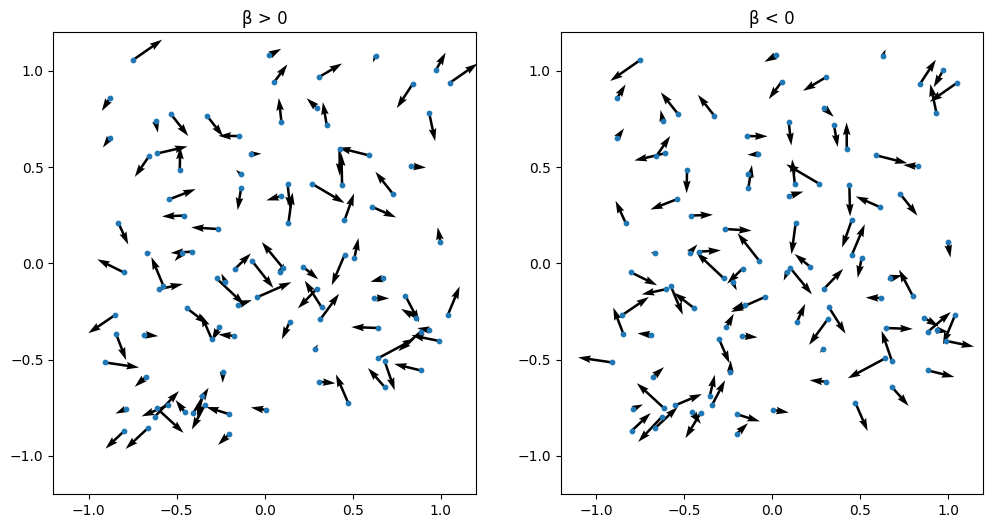
\includegraphics[width=0.8\linewidth]{tcc//img/100corpos_betas.png}
    \caption{Posições e momentos lineares em um problema de 100 corpos com todas as integrais primeiras nulas para os dois valores de $\beta$.}
    \label{fig:vi-betas}
\end{figure}




%%%%%%%%%%%%%%%%%%%%%%%%%%%%%%%%%%%%%%
\subsection{Condições de estabilidade}\label{subsection:condicoes_aarseth}
Em busca de um sistema de unidades padrão que permitisse a comparação de resultados obtidos por diferentes pesquisadores do PNCG, \citep{Hnon1972, Heggie} propõem utilizar o seguinte:
\begin{equation*}
    G = 1, \quad
    M = 1, \quad
    R_V = 1.
\end{equation*}
sendo $R_V$ o raio de virial. Isso significa que temos o seguinte, conforme equação (\ref{eq:raio_virial}):
\begin{equation*}
    V \approx - \dfrac{G M^2}{2 R_V} = - \dfrac{1}{2},
\end{equation*}
e pelo Teorema do Virial (Teorema \ref{teorema:virial}) para uma relação de equilíbrio instantânea:
\begin{equation*}
    T = - \dfrac{1}{2} V \approx \dfrac{1}{4} 
    \Rightarrow
    E = - \dfrac{1}{4}.
\end{equation*}

Para sistemas com essas condições iniciais, é esperado que, com alguma regularização em uso (como o amortecimento do potencial, por exemplo), o sistema fique limitado - ou seja, \textit{estável} -, ao menos temporariamente.

Os testes apresentados nas próximas subseções nos quais as massas são iguais e somam 1 utilizam as condições de Hénon.
